
\documentclass[a4paper]{report}
\usepackage[utf8x]{inputenc}
% bibliography
\usepackage{natbib}
%\bibpunct{[}{]}{,}{a}{}{;}

\usepackage{fancyheadings}
\usepackage{iamdip}
\usepackage[pdftex]{graphicx}
% ignore missing images
%\usepackage[demo]{graphicx}
\usepackage[labelfont=bf, font={sf,normalsize}, margin=0.5cm]{caption}
\usepackage{caption}
\usepackage{subcaption}
\usepackage{amsmath}
\usepackage{marvosym}
\usepackage{amssymb}
\usepackage{amsfonts}
\usepackage{url}
\usepackage{hyperref}
\usepackage[procnames]{listings}
\usepackage{chngpage}
\usepackage{rotating}
\usepackage{wrapfig}

% For notation table
\usepackage{tabulary}
\usepackage{booktabs}

\usepackage{here}

\headrulewidth 0.5pt \addtolength{\headheight}{5pt}
\lhead[\fancyplain{}{\rm\thepage}]{\fancyplain{}{\rightmark}}
\rhead[\fancyplain{}{\leftmark}]{\fancyplain{}{\rm\thepage}}
\cfoot{}

\graphicspath{{Figures/}}

\newcommand{\T}{^\text{T}}

% for fancy todo
\usepackage{todonotes}
\newcommand{\todoRef}{\todo[color=green!20]}
\newcommand{\todoEnglish}{\todo[color=red!20]}
\newcommand{\todoFormat}{\todo[color=blue!20]}
\newcommand{\todoWriteMore}{\todo[color=yellow!40, inline]}
\newcommand{\todoRewrite}{\todo[color=purple!20, inline]}
\newcommand{\todoQ}{\todo[color=blue!20]}

% math definitions, propositions and such
\usepackage{amsthm}
\newtheorem{definition}{Definition}
\newtheorem*{rules}{Rules}
\newtheorem*{example}{Example}
\newtheorem*{assertion}{Assertion}

% tree packages and basic settings
\usepackage{tikz}
\usetikzlibrary{arrows,shapes,positioning,shapes.geometric,fit}
\usepackage{xcolor}
\tikzset{
treenode/.style = {align=center, inner sep=0pt, text centered,
font=\sffamily},
arn_n/.style = {treenode, circle, white, font=\sffamily\bfseries, draw=black,fill=black, text width=1.5em},% arbre rouge noir, noeud noir
arn_r/.style = {treenode, circle, black, draw=blue, text width=1.5em, very thick},% arbre rouge noir, noeud rouge
arn_w/.style = {treenode, circle, draw=black, text width=1.5em, very thick},% arbre rouge noir, noeud rouge
arn_x/.style = {treenode, rectangle, draw=black, minimum width=0.5em, minimum height=0.5em},% arbre rouge noir, nil
subtree/.style  = {regular polygon, regular polygon sides=3, draw=black, align=center, minimum size=1cm, anchor=center}
}

\newcommand{\newCommandName}{text to insert}
%%%%%%%%%%%%%%%%%
% begin document
\begin{document}

\pagestyle{fancyplain} \thispagestyle{empty}

\title{A Proof Search Implementation in Python\\ for Justification Logic}
\author{Judith Fuog}
\betreuer{Prof.\ Dr.\ Thomas Studer}
\ort{Bern}
\datum{2015}


\pagenumbering{roman} \setcounter{page}{1}
\maketitle

\newpage
\thispagestyle{empty}
\vspace{8cm}
\noindent
{\centerline {\bf \large Abstract}}
\vspace{1cm}
\label{abstract}
%!TEX root = ../bachelors_thesis.tex

Justification Logic as part of the larger field modal logic provides some means to give more information about a proof. Information and researches about this topic are currently still rather limited. 

However the thesis presented here does not concern itself with the theoretical details of Justification Logics but focus on a proof search approach for this specific logic.  The implementation is done in the language Python.

\pagenumbering{roman} \setcounter{page}{1}
\tableofcontents


\newpage{\pagestyle{empty} \cleardoublepage}

% Hauptdokument
\pagenumbering{arabic} \setcounter{page}{1}
\pagestyle{fancy}


%!TEX root = ../bachelors_thesis.tex
\chapter{Introduction}

\section{Motivation}
\todoWriteMore{What's the motivation behind it? Not \textbf{MY} motivation, but the scientific motivation.}

\section{Goal}
\par
The initial goal was to extend an existing proof search engine Z3 [\cite{z3}] such that it could also handle Justification Logic. Deeper investigation into that project revealed that to make it handle also Justification Logic the given interface in Python would not work. Instead it would have to be look into the core of the programm which is written in C. The expenses it would require to get so much deeper into the material that the actual indented work would be only secondary.
So instead of extending Microsoft Research project the actual goal changed to implementing a simplified proof search for Justification Logic. It meant that the implementation would be easier since it does not depend on anything else anymore. As a downside a lot of the functionallity that was hoped go get from Z3 would have to be implemented as well or left out.

\par The program should satisfy to following conditions: \todoQ{Should this really be here in this chaper?}

\begin{itemize}
	\item[Input] The formula to be proven as well as a list of formulas needed for the proof is given as string. It may be presumed that the string is exactly formatted in the way needed. It must not be checked for syntax error or general typing mistakes.
	\item[Output] A simple \emph{True} or \emph{False} for the provability of the formula. \footnote{Optional the output could give information about how a proof was found if the formula is provable.}
\end{itemize}

\section{Overview}
The second chapter will present a short introduction to Justification Logic, but will go only as deep as needed to understand the problem as well as the develop algorithm.
\par
The heart of the third chapter will introduce the algorithm used in the \todoFormat{j-logic} program. Since this thesis concerns itself more with the practical side of implementation and not the theoretical side of mathematical logic theory there will be little proof here but instead many example to show how the algorithm works.
\par
Finally the last chapter will discuss the result of the work and give some ideas about how the work of a Justification Logic proof search implementation could be improved. 

\chapter{Justification Logic}
\label{chap: Justification Logic}
%!TEX root = ../bachelors_thesis.tex
The theory of justification logic as it is used here requires little knowledge of the wide field of modal logic apart from very basic about logic theory. For the purpose of this proof search a few basic rules and definitions are sufficient to provide the needed knowledge. 

The theory presented here is based mainly on the work of Goetschi~\cite{goet} as well as the older reference Artemov~\cite{art} and also from the homepage \cite{stan}. These definitions and rules given here are not complete to the justification logic. Priority was given to those informations which are vital for the implementation. So however briefly and incomplete the theory is presented here full reference can be found in the named sources. 

\section{Background}
Justification Logic has its origins from the field of modal logic. 
In model logic $\square A$ means that $A$ is \emph{known} or that we have \emph{proof} of $A$. In justification logic the equivalent would be $t:A$ where $t$ is a \emph{proof term} of $A$. This gives us the notion that \emph{knowledge} or \emph{proofs} may come from different sources. Justification logic lets us connect different \emph{proofs} with a few simple operations and thus gives us a better description of the proof. To quote Goetschi~\cite{goet}: It may be said that where in model logic the knowledge is implicit it is explicit in justification logic.

\section{Rules and Definitions}

The language of justification logic is given here in a more traditional form with \emph{falsum} and \emph{implication} as primary propositional connectives. Although for the work done with this implementation only the implication is used and the falsum has been ignored. Also not all available syntactic objects are introduces here but only those implemented.

\begin{definition}\label{justification_terms} Apart from formulas, the language of justification logics have another type of syntactic objects called \emph{justification terms}, or simply \emph{terms} given by the following grammar:
\[
	t::=  \;c_{i}^{j}\; |\; x_i \;|\; \bot \; |\; (t \cdot t)\; |\; (t+t)\; |\; !t
\]
where $i$ and $j$ range over positive natural numbers, $c_{i}^{j}$ denotes a (justification) \emph{constant} of level $j$, and $x_i$ denotes a (justification) \emph{variable}.

The binary operations $\cdot$ and $+$ are called \emph{application} and \emph{sum}. The unary operation $!$ is called \emph{positive introspection}.
\end{definition}

\begin{rules}\label{rules} 

\begin{itemize} Application, sum and positive introspection respectively.

	\item[C1] $t:(F \rightarrow G), \; s:F \vdash (t \cdot s): G$\label{rule:c1}
	\item[C2] $t:F \vdash (t +s):F, \; s:F \vdash (t+s):F$\label{rule:c2}
	\item[C3] $t:F \vdash \; !t:(t:F)$\label{rule:c3}
\end{itemize}

\end{rules}

Formulas are constructed from propositional letters and boolean constants in the usual way with an additional clause: if $F$ is a formula and $t$ a term, then $t:F$ is also a formula.

\begin{definition}\label{justification_formulas} \emph{Justification formulas} are given by the grammar:
\[
A ::= P_i\;|\;(A \rightarrow A) \;|\; (t:A)
\]
where $P_i$ denotes a proposition, as in the modal language, and $t$ is a justification term in the justification language.
\end{definition}

This is almost all we need for the proof search of a (justification) formula. The last definition gives us a reference for the proof constants.

\begin{definition}\label{cs-def} A constant specification, \emph{CS}, is a finite set of formulas of the form $c:A$ where $c$ is a proof constant and $A$ is a axiom of Justification language.
\end{definition}

The axioms mention in this definition are \emph{C1-C3} in addition to $t:(F \rightarrow F)$ and the Axioms of the classical propositional logic in the language of LP.



\newpage{\pagestyle{empty} \cleardoublepage}

\chapter{A Divide and Conquer Algorithm}
\label{chap: Algorithm A Divide and Conquer Approach}
%!TEX root = ../bachelors_thesis.tex
\section{The Core Idea}
In my earliest attempts the methods of my algorithm had the tendency to explode with the number of \texttt{if-else} and \texttt{switch} statements. Also they were always very deep nestled. It was sheer impossible to keep track of what had to be done where under which circumstances and whenever I though I had it I found more cases that needed takes special care of. What I really needed was a strategy. I started experiencing with the proof terms of the justification formula, trying to take it somehow apart and restructure the formula in a way that would make handle it easier. I was looking for something like the conjunctive normal form (CNF) and the way how it is used in proof search calculus\footnote{\emph{Proof Search Calculus} as it is introduced in \cite{jaeg}}. Indeed I found a way that allows me to \emph{divide} a justification formula in disjunctive formulas where proving only one of them is also proof for the whole justification formula. The main advantage gained from dividing the justification formula is that the resulting formula have far less variety in the manner of their operations and thus are easier to further analyze.

The comprehension that my approach follows a classic \emph{Divide and Conquer} approach came to me only later when I started \emph{conquering}. The algorithm presented here may not be a model of \emph{Divide and Conquer} but similarities cannot be denied. For that reason I have structured this chapter accordingly.

\medskip

There are two major steps in the divide part of this algorithm. First the justification formula itself will be split into several smaller pieces and adjusted. Second each of those smaller pieces called \emph{atoms} is also being be taken apart so that only their proof constant with a corresponding proof term containing variables remains. The pair of proof constant and proof term will be called \emph{must}\footnote{They are called \emph{musts} in the algorithm because we have to find a match for every single one of them or else the atom is not provable.}.

The conquer step first handles the \emph{musts} of one atom, trying to find a valid match for every \emph{must} in the constant specification list and then evaluates from the results of each \emph{atom} the provability of the originally given justification formula.

\section{Divide}\label{chap:Algorithm.divide}
The aim of this first step is to split it into smaller pieces and standardize them to make it easier to get the \emph{musts}.

\subsection{Atomize a Justification Formula}\label{chap:Algorithm.atomize}
\begin{definition}[atomic]
	A formula or term is called \textbf{atomic} if it fulfills the following conditions:
	\begin{itemize}
		\item The term contains no sum operations.
		\item A introspection operation can neither be the top operation of a term nor be the left operant of a application operation.
	\end{itemize}	
\end{definition}
To make the content presented here more understandable the following example will illustrate the steps taken.\footnote{It is on purpose that the \emph{justification term} is by far more complicated than statement $b:F$ that follows the \emph{justification term}. As far as this algorithm goes the complexity of the statement is of no further consequence and thus is kept as simple as possible to allow a easier overview.}

\subsubsection{Sumsplit}
\label{sumsplit}
From the sum rule of justification logic in \ref{rules} it follows that checking for provability in a formula where the top operation is a sum is equal to checking either operant of the sum and if any of it is provable so is the original formula.

\begin{align}\label{ss1}
	(s+t):F \quad \Rightarrow \quad s:F \lor t:F
\end{align}

%!TEX root = ../bachelors_thesis.tex
\begin{figure}[H]
\begin{center}
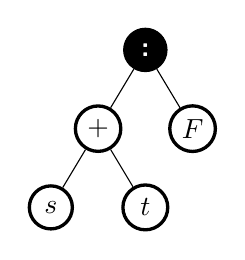
\begin{tikzpicture}[level distance=1cm,
  level 1/.style={sibling distance=1.2cm}]
	\node [arn_n]{:}
	  child {node [arn_w]{\(+ \)}
	  	child {node [arn_w] {$s$}}
	  	child {node [arn_w] {$t$}}
	  }
	  child {node [arn_w]{$F$}};
\end{tikzpicture}
\hspace{2cm}
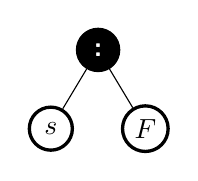
\begin{tikzpicture}[level distance=1cm,
  level 1/.style={sibling distance=1.2cm}]
	\node [arn_n]{:}
	  child {node [arn_w]{\(s\)}}
	  child {node [arn_w]{$F$}};
\end{tikzpicture}
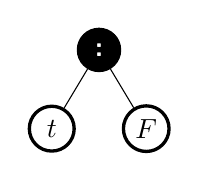
\begin{tikzpicture}[level distance=1cm,
  level 1/.style={sibling distance=1.2cm}]
	\node [arn_n]{:}
	  child {node [arn_w]{\(t \)}}
	  child {node [arn_w]{$F$}};
\end{tikzpicture}
\caption{Example of a simple sumsplit.}
\end{center}
\end{figure}
\todo{Caption}

This is also true for formulas where sum is not the top operation. Here $X$ denotes a arbitrary \emph{justification term}.

\begin{align}\label{ss2}
	(r*(s+t)):F  \quad & \Rightarrow r: X \rightarrow F \land (s+t): X \\
	& \Rightarrow ( r: X \rightarrow F \land s: X ) \lor ( r: X \rightarrow F \land t: X )
\end{align}

%!TEX root = ../bachelors_thesis.tex
\begin{center}
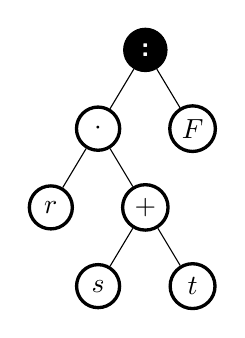
\begin{tikzpicture}[level distance=1cm,
  level 1/.style={sibling distance=2cm},
  level 1/.style={sibling distance=1.2cm}]
	\node [arn_n]{:}
	  child {node [arn_w]{\(\cdot \)}
	  	child {node [arn_w] {$r$}}
	  	child {node [arn_w] {$+$}
		  	child {node [arn_w] {$s$}}
		  	child {node [arn_w] {$t$}}	  		
	  	}
	  }
	  child {node [arn_w]{$F$}};
\end{tikzpicture}
\hspace{1.5cm}
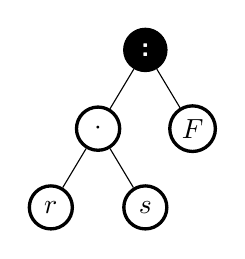
\begin{tikzpicture}[level distance=1cm,
  level 1/.style={sibling distance=1.2cm}]
	\node [arn_n]{:}
	  child {node [arn_w]{\(\cdot \)}
	  	child {node [arn_w] {$r$}}
	  	child {node [arn_w] {$s$}}
	  }
	  child {node [arn_w]{$F$}};
\end{tikzpicture}
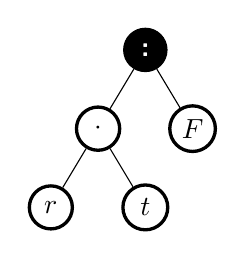
\begin{tikzpicture}[level distance=1cm,
  level 1/.style={sibling distance=1.2cm}]
	\node [arn_n]{:}
	  child {node [arn_w]{\(\cdot \)}
	  	child {node [arn_w] {$r$}}
	  	child {node [arn_w] {$t$}}
	  }
	  child {node [arn_w]{$F$}};
\end{tikzpicture}
\end{center}
\todo{Caption}

\subsubsection{Simplify Introspection}
In this step we try to get rid of any introspection operation that is the first operation of a formula. Either the introspection can be removed and the formula simplified or else the formula is not provable at all and can be discarded.

Derived from the application rule in \ref{rules} we get the following:

\begin{align}\label{sb}
	!t:(t:F) \quad & \Rightarrow t: F
\end{align}

%!TEX root = ../bachelors_thesis.tex
\begin{figure}[H]
\begin{center}
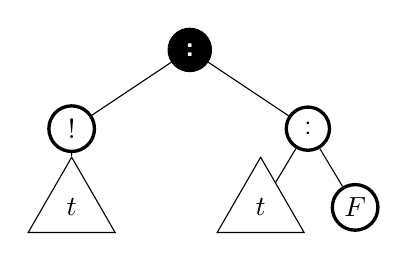
\begin{tikzpicture}[level distance=1cm,
  level 1/.style={sibling distance=3cm},
  level 2/.style={sibling distance=1.2cm}]
	\node [arn_n]{:}
	  child {node [arn_w]{\(! \)}
	    child[right] {node [subtree] {$t$}}
	    }
	  child {node [arn_w]{:}
  		child {node [subtree] {$t$}}
  		child {node [arn_w] {$F$}}
  		};
\end{tikzpicture}
\hspace{2cm}
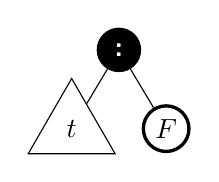
\begin{tikzpicture}[level distance=1cm,
  level 1/.style={sibling distance=1.2cm}]
	\node [arn_n]{:}
	  child {node [subtree]{\(t \)}}
	  child {node [arn_w]{$F$}};
\end{tikzpicture}
\end{center}
\caption{Example of a simplification of a introspection.}
\end{figure}
\todo{Caption}

Speaking in the manner of a syntax tree it needs to be checked, if the child of the introspection operation is identical with the left child of the right child of the root. In that case the formula can be simplified to right child of the root only. Else there is no way to resolve the introspection operation and the formula has to be discarded.

\subsubsection{Remove Contradicting Introspection}
This last step in atomizing the formula proved to be on of the hardest to realize. Only countless examples support the claim that the introspection operation must not be the direct left child of a application operation. In coming to that conclusion it has been helpful that no sum operation could make the situation more complex. Because of this and also the fact that a introspection operation is never the top operation in a formula it is guarantied that a introspection operation must be either a right child or a left child of a application operation.

\begin{align}\label{bb}
	& ((!s)\cdot t):F  \quad \Rightarrow \exists X_1 : (!s): (X_1 \rightarrow F) \quad \land \quad t: X_1\\
	& (!s): (X_1 \rightarrow F)  \quad \Rightarrow \exists X_2 : (!s):(X_1 \rightarrow F) = (!s):(s:X_2)
\end{align}\todo{Make this look more like the ones following below.}
The last line gives a contradiction since there is no possible $X_2$ that would fulfill the condition of $X_1 \rightarrow F = s:X_2$.

\begin{assertion}[Tree Version]
A introspection operation that is the direct left child of a application operation causes the whole term to be invalid (unprovable), given that the term is without sum operations and no introspection operation at the top.
\end{assertion}

%!TEX root = ../bachelors_thesis.tex
\begin{figure}[H]
\begin{center}
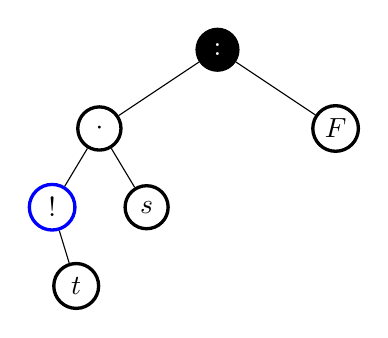
\begin{tikzpicture}[level distance=1cm,
  level 1/.style={sibling distance=3cm},
  level 2/.style={sibling distance=1.2cm}]
	\node [arn_n]{$:$}
	  child {node [arn_w]{\(\cdot \)}
	    child {node [arn_r] {$!$}
	    		child[right] {node [arn_w] {$t$}}
	    	}
	    child {node [arn_w] {$s$}}
	    }
	  child {node [arn_w]{$F$}};
\end{tikzpicture}
\hspace{2cm}
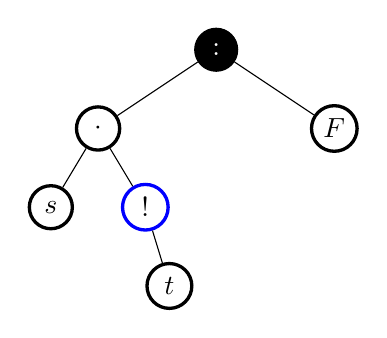
\begin{tikzpicture}[level distance=1cm,
  level 1/.style={sibling distance=3cm},
  level 2/.style={sibling distance=1.2cm}]
	\node [arn_n]{$:$}
	  child {node [arn_w]{\(\cdot \)}
	    child {node [arn_w] {$s$}}
	    child {node [arn_r] {$!$}
	    		child[right] {node [arn_w] {$t$}}
	    	}
	    }
	  child {node [arn_w]{$F$}};
\end{tikzpicture}
\end{center}
\caption{The left tree shows an introspection that gives a contradiction, while the right tree is valid.}
\end{figure}

\par
This concludes the \emph{atomization} of one formula to many simple formulas which can be checked for provability individually. An atomized formula now consists only of application operations and valid introspection operations. The next section will show what further steps are needed to check one atomized formula for its provability.

\subsection{Get the Must Terms}\label{chap:Algorithm.musts}
To check a justification formula for its provability we need to look up the justification constant from the formula in the constant specification list (from now on called \emph{cs-list} for brevity) and compare the justification term with the term we find there.

The operation rules which were presented in chapter \ref{rules} gives us the instruction how we can take a formula apart to look the individual proof term up in the cs-list. The rule for the sum operation was already used in the previous steps for the \texttt{sumsplit} in \ref{sumsplit}.

Each application operation in a term adds one variable and a introspection operation replaces an existing variable\footnote{The variables we get from constructing the \emph{musts} are called \emph{X-wilds} in the source code in contrast to the variables that might occur in the \emph{cs}-list which are refered to \emph{Y-wilds} respectively.} with a new combined with a proof constant. 

So for a term like this $(a \cdot (!b)) \cdot c):F$ the following will be evaluated:

\begin{equation}\label{musts}
\begin{split}
	(a \cdot (!b)) \cdot b):F \\
	& \Rightarrow a \cdot (!b):  X_1 \rightarrow F \\
	& \Rightarrow b:  X_1
\end{split}
\end{equation}
\begin{equation}\label{musts1}
\begin{split}
	(a \cdot (!b)): X_1 \rightarrow F \\
	& \Rightarrow a: X_2 \rightarrow (X_1 \rightarrow F)\\
	& \Rightarrow !b: X_2
\end{split}
\end{equation}
\begin{equation}\label{musts2}
\begin{split}
	!b: X_2 \\
	& \Rightarrow X_2 = b:X_3
\end{split}
\end{equation}

$X_2$ will be replaced by $b:X_3$ so our final \emph{musts} for $(a*(!b))*c):F$ looks like this: 
\begin{equation}\label{must-list}
 [ \bigl( a, ((b:X_3) \rightarrow (X_1 \rightarrow F)) \bigr) , \bigl( b, X_1 \bigr) , \bigl( b, X_3 \bigr) ] 
\end{equation}

As can be seen in this example a proof constant may have more than one term that needs to be looked up in the cs-list.

\section{Conquer}

Once that the \emph{musts} have been obtained we can search the cs-list for terms that match it. Since a \emph{must} usually consists of variables that are not determined it is possible that we get more then one match per proof term. Also since the cs-list allows terms that contain variables as well this imposes further conditions on the possible choice of the term of a proof term. All those possibilities and conditions are collected when comparing the musts with the cs-list.

Then in the second and most important step in the conquer part those conditions will be merged. It will be checked if there is a possible combination from the given options such as the atomized formula is provable. It is then only a small step to collect the results of all other atoms of the original formula to determine the provability of the original formula. 

Throughout this section the words \emph{conditions} and \emph{configurations} is being used. Since they mean something very similar but not the same the definition of the usage of those words is presented below:

\begin{definition}[condition]
A \emph{condition} is either on a $X$ variable or on a $Y$ variable. A condition can be a constant, a variable or a term containing constants and/or variables. One variable may have several \emph{conditions} which may contradict each other at certain stages. A \emph{condition} may not contain the variable on which the \emph{condition} is in its term.\\
A set of conditions is per proof constant of a \emph{must} at first but it may also be a set for several proof constant after the conditions have been merged.
\end{definition}

\begin{definition}[configuration]
A \emph{configuration} is a special case of a \emph{condition}. It is also on a $X$ or $Y$ variable but a configuration contains only constants and no more other variables. There can only be one configuration per variable as it would contradict any other configuration.\\
\end{definition}

\subsection{Matching with CS-List}
Central for the whole conquer part is the procedure of comparing two formulas and giving a useful result. This is needed when we first try to match our \emph{musts} with what we find in the cs-list and later again when we assemble the different conditions and merge them together.

For one atom we have now several \emph{musts}, each of these musts corresponds to a proof constant and holds a term usually made up from at least one variable. On the other hand the terms we find within the cs-list are not only terms with constants but also axioms that can contain variables as well. This means that the result of a comparison of such two formulas are conditions that apply to certain variables. 

If we compare the term $(X_2 \rightarrow (X_1 \rightarrow F))$ of a \emph{must} with the term $(Y_1 \rightarrow (Y_2 \rightarrow Y_1)$ from the cs-list for example, we get the following conditions:
\begin{align*}
	X_1 &: \{Y_2\} \\
	X_2 &: \{Y_1\} \\
	Y_1 &: \{X_2, F\} \\
	Y_2 &: \{X_1\} 
\end{align*}

Which can be shorted without loosing any informations to\footnote{This is only one of many options to shorten the conditions, another option would be $Y_1: \{X_2, F\}, Y_2:\{X_1\}$.}:

\begin{align*}
	X_1 &: \{Y_1\} \\
	X_2 &: \{F\} \\
	Y_2 &: \{F\}
\end{align*}

For every entry in the cs-list that we compare to our \emph{must} gives us a set of conditions for the occurring variables. Each set represents a possible proof for one \emph{must}, but since all \emph{musts} have to be proofed and since they contain variables that also occur in other \emph{musts} the sets of conditions of all \emph{musts} of a atom have to be merged together.

\subsection{Merging Conditions to Configurations}
Suppose we have \emph{musts} $m_1, m_2, ..., m_n$ for a certain atom. From the previous step each of these $m_i$ has at least\footnote{If there is no entry in the cs-list that matches the criteria of a \emph{must} it makes the whole atom unprovable.} one set of conditions for its variables, possibly more. Our aim is to find one set of conditions for each \emph{must} such that when we put all those conditions together we have not contradiction. This gives us the final configuration of the $X$ variables\footnote{We are only concerned for the \emph{X-wilds} but we still need to tag the \emph{Y-wilds} along.}.

Let us say we have the \emph{musts} $m_k$ and $m_{k+1}$ and the following sets of conditions: For $m_k$ we find only one set, for $m_{k+1}$ we shall have two.


\begin{align*}
	m_k: [	& \{X_1: \{(A \rightarrow X_3)\}, X_2: \{A\}\}]\\
	m_{k+1}: [	& \{X_1: \{(X_2 \rightarrow B)\}, X_4: \{X_3\}\},\\
			& \{X_1: \{X_2\}, X_4: \{B\}\}]
\end{align*}

We see that the first set of $m_j$ is compatible with the set of $m_i$ and the second set of $m_j$ is not.

To archive the same result with the algorithm the two conditions are first simply joined, ignoring possible contradictions, giving us two new sets of conditions.

\begin{align*}
	& \{	X_1: \{(A \rightarrow X_3), (X_2 \rightarrow B)\}, 
						X_2: \{A\}\}, 
						X_4: \{X_3\}\},\\
					& \{X_1: \{(A \rightarrow X_3), X_2\},
						X_2: \{A\}\}, 
						X_4: \{B\}\}\\
\end{align*}



For the first set of condition we get from the join, resolving the conditions for $X_1$ gives us $X_2:A$ which also fits with the condition for $X_2$ that is already present. Further $X_3: B$ gives us also $X_4: B$. If the variables that we find in $m_i$ and $m_j$ are all that occur in all other \emph{musts} of the atom we have found a configuration for the variables, thus proving the atom.

\begin{align*}
	& \{X_1: \{(A \rightarrow B)\}, X_2: \{A\}\}, X_3: \{B\}, X_4: \{B\}\}\\
\end{align*}

In the second set resolving the conditions does not work out. From $X_1$ we get that $X_2: (A \rightarrow X_3)$ which is not compatible with the existing condition on $X_2$ that states $X_2: A$. Consequently the second set is discarded. If the first set had failed as well there would be no proof for this atom.


\subsection{Analyzing the Results}
In the end we get for each atom from the original formula a set of possible configurations. A set may contain several configurations, meaning that the variables of this atom can be configured differently, it may contain only one configuration, meaning that there is only one possible configuration or there may be none at all, meaning that there are no valid configurations for the variables of this atom thus making it unprovable.

Sine proofing one atom of a formula proves the whole formula, the last step taken by the algorithm is to check if at least one atom is provable. In theory the algorithm could stop as soon as it finds the first provable atom, but in this implementation is checks all the atoms and aside from giving a simple \texttt{True} or \texttt{False} it provides also the configuration(s) of the variables for all provable atoms.



\bigskip
\par This concludes the whole divide and conquer chapter. I personally have found it rather easy to understand the individual steps but difficult not to get lost in the overall view. For that reason chapter \ref{chap: Example} will cover one single example designed to show all aspects of the algorithm and run it through from start to end to help understanding it better.



\chapter{Implementation}
\label{chap: Implementation}
\definecolor{keywords}{RGB}{255,0,90}
\definecolor{comments}{RGB}{0,0,113}
\definecolor{red}{RGB}{160,0,0}
\definecolor{green}{RGB}{0,150,0}
\lstset{language=Python, 
        basicstyle=\ttfamily\small, 
        keywordstyle=\color{keywords},
        commentstyle=\color{comments},
        stringstyle=\color{red},
        showstringspaces=false,
        identifierstyle=\color{green},
        procnamekeys={def,class},
        linewidth=8cm} 
%!TEX root = ../../bachelors_thesis.tex
\section{Implementation and Example}
\begin{example}
\[
	((((a*b)*(!b))+((!b)+c))+((!b)*d)):(b:F)
\]
\end{example}

\subsection{Model and Build}
\subsection{Example}

\chapter{Example}
\label{chap: Example}
%!TEX root = ../bachelors_thesis.tex
In this chapter I walk through a complete example covering as many special cases as possible. As such, the justification term we will look at is rather complicated but it will also show how nicely it can be broken down in more simpler atoms.

\section{Initialization}
The algorithm takes a formula $f$ and a cs-list as input. The data presented here is in the same form as it would be entered into the program. Therefore the cs-list is a \emph{python} dictionary and not simple list of pairs and there are more brackets explicitly written then required by convention.

\begin{align}\label{eq:f}
f = (((!(a+c))+((a+(!a))\cdot (b\cdot (!c)))):(c:F))
\end{align}

\begin{equation}\label{cs}
\begin{split}
	cs = \{& a: [(H \rightarrow (c:F)), ((E \rightarrow (c:D)) \rightarrow (c:F)), (E \rightarrow (c:D))],\\
	& b: [((c:F) \rightarrow H), ((c:D) \rightarrow (a:F)), ((H \rightarrow G) \rightarrow H), (Y_1 \rightarrow (Y_2 \rightarrow Y_1))],\\
	& c: [(c:F), G, D, (G \rightarrow F)]\}
\end{split}
\end{equation}




\section{Walking in Trees: Atomize}

The given formula $f$ is transformed into a syntax tree using \texttt{parse\_formula} of \texttt{Tree}. 

\subsection{Sumsplit}
Our first step is to split our formula for every sum we encounter.
\begin{equation*}
	(((!(a
    \tikz[baseline]{\node[fill=red!20,anchor=base] (t1){$+$};} c))
    \tikz[baseline]{\node[fill=red!20,anchor=base] (t2){$+$};} ((a
    \tikz[baseline]{\node[fill=red!20,anchor=base] (t3){$+$};} (!a))\cdot (b\cdot (!c)))):(c:F))
\end{equation*}

%!TEX root = ../../bachelors_thesis.tex
\begin{figure}[H]
\caption{Syntax tree of given formula $f$ before it is atomized.}
\begin{center}
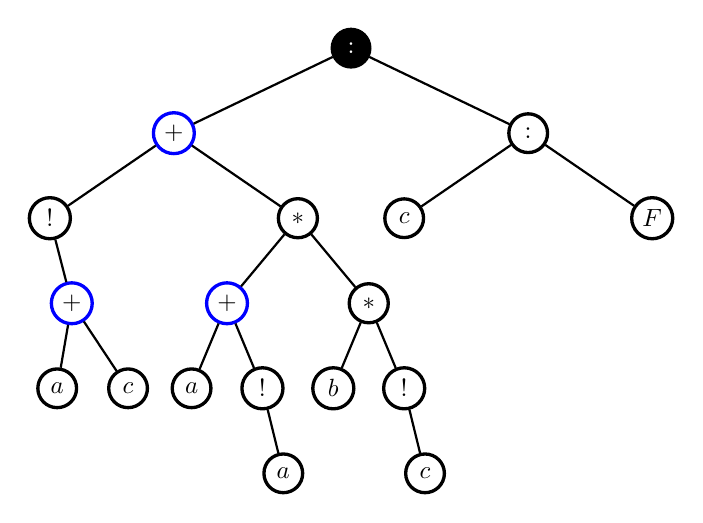
\begin{tikzpicture}[level distance=1.2cm,
  level 1/.style={sibling distance=5cm},
  level 2/.style={sibling distance=3.5cm}, 
  level 3/.style={sibling distance=2cm},
  level 4/.style={sibling distance=1cm},
  level 5/.style={sibling distance=1.5cm}, thick,scale=0.9, every node/.style={scale=0.9}]
	\node [arn_n]{$:$}
	  child {node [arn_r]{\(+ \)}
	    child {node [arn_w] {$!$}
	    	child[right] {node [arn_r] {$+$}
	    		child {node [arn_w] {$a$}}
	    		child {node [arn_w] {$c$}}
	    		}
	    	}
	    child {node [arn_w] {$*$}
	    	child {node [arn_r] {$+$}
	    		child {node [arn_w] {$a$}}
	    		child {node [arn_w] {$!$}
	    			child[right] {node [arn_w] {$a$}}
	    			}
	    		}
	    	child {node [arn_w] {$*$}
	    		child {node [arn_w] {$b$}}
	    		child {node [arn_w] {$!$}
	    			child[right] {node [arn_w] {$c$}}
	    			}
	    		}
	    	}
	    }
	  child {node [arn_w]{$:$}
	  	child {node [arn_w] {$c$}}
	  	child {node [arn_w] {$F$}}
	  };
\end{tikzpicture}
\end{center}
\end{figure}


The \texttt{sum\_split} from \texttt{Tree} will give us the following terms in form of a list. 

\begin{equation}\label{eq:sp_i}	
	((!a):(c:F))
\end{equation}
\begin{equation}\label{eq:sp_ii}	
	((!c):(c:F))
\end{equation}	
\begin{equation}\label{eq:sp_iii}	
	((a \cdot(b\cdot (! c))):(c:F))											
\end{equation}
\begin{equation}\label{eq:sp_iv}	
	(((! a)\cdot(b\cdot (! c))):(c:F))												
\end{equation}
Some of those will eventually be the atoms for $f$, but before they can become atoms of $f$ they need to be simplified and checked.

\subsection{Introspections}
We now look at the terms to discard any that have a introspection operation that is the left child of a multiplication or if there are proof terms that start with a introspection operation and cannot be simplified. If they can be simplified they will of course not be discarded but simplified.

\subsubsection[First term]{Term (\ref{eq:sp_i})}
In this term we find a introspection which is valid, since it is not a left child of a multiplication, but trying to simplify the term shows us that it cannot be resolved thus letting us discard this term.

\begin{equation*}
	((\tikz[baseline]{\node[fill=red!20,anchor=base] (t1){$!$};}a):(c:F)) 
\end{equation*}

\subsubsection[Second term]{Term (\ref{eq:sp_ii})}
As before the introspection for the term is valid and in contrast to the previous example the term here can be simplified, giving us our first \emph{atom} for formula $f.$

\begin{equation}\label{eq:a_1}
	\begin{split}
	((\tikz[baseline]{\node[fill=red!20,anchor=base] (t1){$!$};} c):(c:F)) & \Rightarrow \\
	& a_1 := (c:F)
	\end{split}
\end{equation}

\subsubsection[Third term]{Term (\ref{eq:sp_iii})}
In this term we find the introspection operation neither a left child of a multiplication nor as top operation of the proof term and thus we have our second \emph{atom}.

\begin{equation}\label{eq:a_2}
	\begin{split}
	((a \cdot(b\cdot (\tikz[baseline]{\node[fill=red!20,anchor=base] (t1){$!$};} c))):(c:F))	 & \Rightarrow \\
	& a_2 := ((a \cdot(b\cdot (! c))):(c:F))
	\end{split}
\end{equation}

\subsubsection[Fourths term]{Term (\ref{eq:sp_iv})}
Finally this term has two introspections of which the first is the left child of a multiplication and thus makes the term invalid. The second introspection would be valid, but the first term causes the whole subterm to be discarded.

\begin{equation*}
	(((
	\tikz[baseline]{\node[fill=red!20,anchor=base] (t1){$!$};} a)\cdot(b\cdot (
	\tikz[baseline]{\node[fill=red!20,anchor=base] (t1){$!$};} c))):(c:F))
\end{equation*}

\bigskip
This completes the \texttt{atomize} step for the formula $f$ giving us the two atoms $a_1$ and $a_2$. Showing that at least one of those is provable is enough to show that $f$ is provable. 

\section{Getting and Looking up the Musts}

\begin{equation*}
		f = (((!(a+c))+((a+(!a))\cdot(b\cdot(!c)))):(c:F)) 
		\tag{\ref{eq:f}}  
\end{equation*}
We have found the two atoms $a_1$and $a_2$ for the formula $f$. The next step determins the \emph{musts} if needed, matching them against the cs-list and finally merge the possible configurations together to determine if one of the musts is provable.


\begin{equation*}
		a_1 = (c:F) 
		\tag{\ref{eq:a_1}}
\end{equation*}
\begin{equation*}		
		a_2 = ((a \cdot(b\cdot (! c))):(c:F)) 
		\tag{\ref{eq:a_2}}
\end{equation*}

\subsection{Musts}
\subsubsection[First atom]{Atom $a_1$ (\ref{eq:a_1})}
Since $a_1$ consists already only of one proof constant with the corresponding term there is nothing further to to here.
\begin{equation}
	a_1: \quad musts = [(c, F)]
\end{equation}

\subsubsection[Second atom]{Atom $a_2$ (\ref{eq:a_2})}
For $a_2$ we need to take the proof term apart bit by bit. The first operation we take apart is a application. Extracting proof constants from a application proof term us give a \emph{X-wild}. 

Whenever a new X variable appears the $i$ of $X_i$ will simply be increased by one to ensure that it is fresh in the formula.

\begin{align*}\label{eq:musts1_a_2}
		((a \cdot(b\cdot (! c))):(c:F)) \Rightarrow & \\
		 a : &(X_1 \rightarrow (c:F)) \\
		 (b\cdot(! c)): &X_1
\end{align*}

The proof constant $a$ has been isolated but $(b\cdot(! c))$ still needs to be taken apart further. We repeat the step from above and introduce yet another X variable.

\begin{align*}
	(b\cdot(! c)): X_1 \Rightarrow & \\
	b : & (X_2 \rightarrow X_1) \\
	(! c) : & X_2
\end{align*}

Now $b$ has been isolated as well, leaving $(! c)$ as the only unresolved proof constant. Having a introspection in this situation results in a new X variables in combination with the proof term which will replace a previous X variables.

\begin{equation*}
	\begin{split}
		(! c) : X_2 & \Rightarrow \\
		& X_2 = (c:X_3)
	\end{split}	
\end{equation*}

This finally gives us all the \emph{musts} for $a_2$. As can be seen belove the \emph{X-wild} $X_2$ has been replaced by $(c:X_3)$.
\begin{equation}\label{eq:a2_musts}
	[(a, (X_1 \rightarrow (c:F))), (b, ((c:X_3) \rightarrow X_1)), (c, X_3)]
\end{equation}

Note that the same proof constant may be in more than one of the \emph{musts} for one \emph{atom}. 

\subsection{Using the CS-List}
We now have to look up all \emph{musts} of each atom the see if the atom is provable.

\begin{align*}
	cs = \{& a: [(H \rightarrow (c:F)), ((E \rightarrow (c:D)) \rightarrow (c:F)), (E \rightarrow (c:D))],\\
	& b: [((c:F) \rightarrow H), ((c:D) \rightarrow (a:F)), ((H \rightarrow G) \rightarrow H), (Y_1 \rightarrow (Y_2 \rightarrow Y_1))],\\
	& c: [(c:F), G, D, (G \rightarrow F)]\}
	\tag{\ref{cs}}
\end{align*}

The atom $a_1$ (\ref{eq:a_1}) is not provable, since its only \emph{must} $c:F$ cannot be found in the cs-list.

The other atom $a_2$ (\ref{eq:a_2}) needs a little bit more work. First we select and compare all \emph{musts} of $a_2$ with the corresponding entries in the cs-list and then we need to find a configuration for the variables of the musts, that will fit all \emph{musts}.

\subsubsection[look up proof constant a]{Proof Constant $a$}
Comparing $(X_1 \rightarrow (c:F))$ with all entries in cs-list for the proof constant $a$ will give us the following two condition sets which are only on the variable $X_1$.
\begin{align}
	(H \rightarrow (c:F)) & \quad \Rightarrow \quad \{X_1: H\} \\ 
	((E \rightarrow (c:D)) \rightarrow (c:F)) & \quad \Rightarrow  \quad \{X_1: (E \rightarrow (c:D))\} \label{condition:a}
\end{align}

\subsubsection[look up proof constant b]{Proof Constant $b$}
For the proof constant $b$ with \emph{must}-term $((c:X_3) \rightarrow X_1)$ we get:
\begin{align}
	((c:F) \rightarrow H) & \quad \Rightarrow \quad \{X_1: F, & X_3: H\}\\ 
	((c:D) \rightarrow (a:F)) & \quad \Rightarrow \quad \{X_1: (a:F), & X_3: D\}\\ 
	((Y_1 \rightarrow (Y_2 \rightarrow Y_1)) & \quad \Rightarrow \quad \{X_1: (Y_2 \rightarrow Y_1), & Y_1: (c:X_3)\} \label{condition:b}
\end{align}
We note that for the last condition set we now have second kind of variable aside from those given in the \emph{must} term. For the moment both kinds of variables are treated exactly the same.

\subsubsection[look up proof constant c]{Proof Constant $c$}
Since the must term for proof constant $c$ is simply $X_3$ we get the following condition sets.
\begin{align}
	(c:F) & \quad \Rightarrow \quad \{X_3: (c:F)\} \\ 
	G & \quad \Rightarrow \quad \{X_3: G\} \\ 
	D & \quad \Rightarrow \quad \{X_3: D\}\label{condition:c} \\ 
	(G \rightarrow F) & \quad \Rightarrow \quad \{X_3: (G \rightarrow F)\} 
\end{align}

\section{Constructing the Final Result}
Now we have several condition sets for each proof constant that have to be put together to a solution.
\subsection{Merging Conditions}
Our goal is to pick one line from each proof constant and that this merged conditions give us a configuration for the X variables. For example we could pick from each the top line, but it is obvious that this is not a solution since $X_3$ can only be either $H$ or $(c:F)$ but not both.

It is clear that not every line of $a$ can be successfully merged with every line of $b$. We see that we can only take those that have the same term for $X_3$ or there is a $Y$-variable. If fact only the two bottom row are compatible, since no entry form $b$ fits $X_1: H$ from $a$ and only $(Y_2 \rightarrow Y_1)$ can be matched with $(E \rightarrow (c:D))$.

\begin{align}
	a \cap b: \quad \{X_1: (E \rightarrow (c:D)), \quad X_1: (Y_2 \rightarrow Y_1), \quad Y_1: (c:X_3)\}
\end{align}

As seen above there are now two conditions that apply to the variable $X_1$. Before we move on and try to merge this set of conditions with one of the lines of $c$ we will resolve the current conditions as far as possible.

Comparing the conditions for $X_1$ we find that $Y_2: E$ and $Y_1: (c:D)$. Since we have already a condition for $Y_1$ that condition is now compared with the new we got from $X_1$ and we will get $X_3: D$. Thus all our variables are now configured:

\begin{align}
	\{X_1: (E \rightarrow (c:D)), \quad X_3: D, \quad Y_1: (c:D), \quad Y_2: E\}
\end{align}

As a consequence of merging line (\ref{condition:a}) from $a$ with line (\ref{condition:b}) from $b$ there is no choice left for the variable and the final result depends on finding a line from proof constant $c$ that matches the value for $X_3$ and as it happens this is the case for line (\ref{condition:c}).


\subsection{Meaning of the Result}
Since we found a valid configuration for the atom $a_1$ (\ref{eq:a_1}) we have shown that the formula $f$ (\ref{eq:f}) is provable. Lets take a step back and see, what the X variables have to do with the provability of $f$.

From our previous step we have a configuration for every variable. We are however only interested in the X variables and do not care further about the $Y$-variables. So we know that $X_1 = (E \rightarrow (c:D))$ and $X_3 = D$. If we replace that in the \emph{musts} for all of the proof constants we get the following:

\begin{equation}
\begin{split}
	a_2: \quad [&(a: ((E \rightarrow (c:D)) \rightarrow (c:F))), \\
	&(b: ((c:D) \rightarrow (E \rightarrow (c:D)))), \\
	&(c: D)]
\end{split}
\end{equation}

As can be seen these entries can all be found precisely like that in the cs-list. Also from those we can reconstruct the term of $a_2$: 

\begin{align}
	& (c:D) \\
	& ((!c):(c:D)) \\
	& ((b\cdot(!c)):(E \rightarrow (c:D)))\\
	& ((a\cdot(b\cdot(!c))):(c:F)) \label{ex:reconstruct}
\end{align}

And with (\ref{ex:reconstruct})) for $a_2$ we have again with what we started right after the atomization step in (\ref{eq:sp_iii}). In the graph below the path with the tree of the atom $a_2$ is highlighted.

%!TEX root = ../../bachelors_thesis.tex
\begin{figure}[H]
\begin{center}
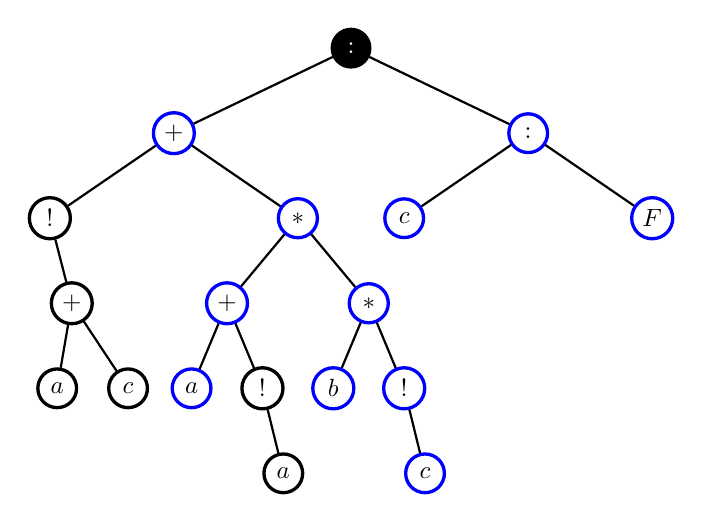
\begin{tikzpicture}[level distance=1.2cm,
  level 1/.style={sibling distance=5cm},
  level 2/.style={sibling distance=3.5cm}, 
  level 3/.style={sibling distance=2cm},
  level 4/.style={sibling distance=1cm},
  level 5/.style={sibling distance=1.5cm}, thick,scale=0.9, every node/.style={scale=0.9}]
	\node [arn_n]{$:$}
	  child {node [arn_r]{\(+ \)}
	    child {node [arn_w] {$!$}
	    	child[right] {node [arn_w] {$+$}
	    		child {node [arn_w] {$a$}}
	    		child {node [arn_w] {$c$}}
	    		}
	    	}
	    child {node [arn_r] {$*$}
	    	child {node [arn_r] {$+$}
	    		child {node [arn_r] {$a$}}
	    		child {node [arn_w] {$!$}
	    			child[right] {node [arn_w] {$a$}}
	    			}
	    		}
	    	child {node [arn_r] {$*$}
	    		child {node [arn_r] {$b$}}
	    		child {node [arn_r] {$!$}
	    			child[right] {node [arn_r] {$c$}}
	    			}
	    		}
	    	}
	    }
	  child {node [arn_r]{$:$}
	  	child {node [arn_r] {$c$}}
	  	child {node [arn_r] {$F$}}
	  };
\end{tikzpicture}
\caption{Syntax tree of formula $f$ with atom $a_2$ hightlighted.}
\end{center}
\end{figure}


\bigskip
This concludes this chapter showing as much as possible with a concise example.

%\newpage{\pagestyle{empty} \cleardoublepage}
%
%\input{Content/guidedImageFiltering}
%
%\newpage{\pagestyle{empty} \cleardoublepage}

\chapter{Conclusion}
%!TEX root = ../bachelors_thesis.tex
Looking back from where I stand now there are many things I would probably have made differently. There is for example a python module called \emph{Pyparser}\todo{Link, Source or anything!}. It allows to create and execute simple grammars and it would have served me to get rid of some of the hard-coded string comparison. An other point I often reflected on it the choice of language. There might have more suitable programming languages for this task then python for example a functional language such as haskell. 

Those are things that I would probably do differently on the other hand there are a lot of things that I could be done to further improve this implementation that have not been possible in this limited time. For user to profit from this implementation it would be necessary g to create a (simple) user interface and even more important it would be necessary to extend this implementation in a way that it may handle any formulas and not just such that use implications. At the very least a negation should be added to archive completeness of the logic structure.

A last point that should be mention is the possible optimization of the implementation of this algorithm. As mention already in the introduction no special care has been given to consider the speed and the algorithm has not been tested for extremely large formulas which might cause the implementation to break due to stack overflow. 
 
%\addcontentsline{toc}{chapter}{\numberline{}List of Tables}
%\listoftables

%\addcontentsline{toc}{chapter}{\numberline{}List of Figures}
%\listoffigures
\addcontentsline{toc}{chapter}{\numberline{}Bibliography}
\bibliographystyle{plain}
%\bibliographstyle{plain}
\bibliography{sources}
%\bibliographystyle{alphadin}
\nocite{*}

\newpage{\pagestyle{empty} \cleardoublepage}
%\chapter*{Authorship}
%\listoftodos

\end{document}